\documentclass[11pt]{article}

\usepackage{graphicx}
\usepackage{listings}
\usepackage{url}
\usepackage{float} % Add this package for the [H] option
\usepackage{listings}
\usepackage{color}

\definecolor{dkgreen}{rgb}{0,0.6,0}
\definecolor{gray}{rgb}{0.5,0.5,0.5}
\definecolor{mauve}{rgb}{0.58,0,0.82}
\usepackage{minted}

\lstset{frame=tb,
  language=Java,
  aboveskip=3mm,
  belowskip=3mm,
  showstringspaces=false,
  columns=flexible,
  basicstyle={\small\ttfamily},
  numbers=none,
  numberstyle=\tiny\color{gray},
  keywordstyle=\color{blue},
  commentstyle=\color{dkgreen},
  stringstyle=\color{mauve},
  breaklines=true,
  breakatwhitespace=true,
  tabsize=3
}

\begin{document}

\begin{titlepage}
    \begin{center}
        
\includegraphics[scale=0.10]{du.png}\par
        \begin{Huge}
            \textsc{University of Dhaka}\par
        \end{Huge}
        \begin{Large}
            Department of Computer Science and Engineering\par \vspace{1cm}
            CSE-3111 : Computer Networking Lab \\[12pt]   
            Lab Report 3 : Implementing File transfer using Socket \\[8pt] Programming and HTTP GET/POST requests
        \end{Large}
    \end{center}     
    \begin{large}
        \textbf{Submitted By:\\[12pt]}
            Name: Md Shamsur Rahman Sami\\[5pt]
            Roll No : 57\\[7pt]
            Name: Md Rakib Hossain\\[5pt]
            Roll No : 55\\[12pt]
        \textbf{Submitted On : \\[12pt]}
            February 08, 2024\\[20pt]
        \textbf{Submitted To :\\[12pt]}
            Dr. Md. Abdur Razzaque\\[12pt]
    \end{large}
\end{titlepage}

\tableofcontents  

\newpage

\section{Introduction}
\subsection{Objectives}

The primary objective of this lab experiment is to delve into the fundamentals of socket programming while emphasizing practical implementation. Through this exercise, participants aim to comprehend the intricacies of creating and managing network sockets, establishing robust connections between client and server applications, and orchestrating data transmission over a network.

A pivotal aspect of this experiment involves the implementation of a client-server communication model, whereby participants craft both client and server applications capable of seamless interaction. This entails mastering the intricacies of socket creation, binding, and listening on the server side, and connecting to the server from the client side. 

Furthermore, the experiment delves into the intricacies of file transfer mechanisms, a quintessential aspect of network communication. Participants navigate the process of reading files from the server and transmitting them to clients, or receiving files from clients and storing them on the server. This involves handling binary data efficiently and ensuring data integrity throughout the transmission process.

An additional focus lies on error handling and robustness, where participants gain insights into implementing mechanisms to address potential issues that may arise during socket communication, such as network disruptions or file transfer errors. By instilling a proactive approach to error handling, participants enhance the reliability and resilience of their socket-based applications, thereby bolstering their proficiency in network programming.

\section{Theory of File Transfer Using Socket Programming and HTTP GET/POST Requests}

This section provides a theoretical overview of implementing file transfer using socket programming and HTTP GET/POST requests. It covers fundamental concepts, protocols, and considerations essential for understanding and implementing file transfer mechanisms.

\subsection{Networking Basics}

\begin{itemize}
  \item \textbf{TCP/IP Protocol Suite:} TCP/IP protocols, including IP, TCP, and UDP, form the backbone of network communication. TCP provides reliable, stream-oriented data transfer, while UDP offers faster, datagram-based communication.
  \item \textbf{Sockets:} Sockets serve as endpoints for network communication, enabling processes to exchange data over a network. Server sockets listen for incoming connections, while client sockets initiate connections to servers.
\end{itemize}

\subsection{HTTP Protocol}

\begin{itemize}
  \item \textbf{Fundamentals:} HTTP operates on a request-response model, with methods like GET and POST for retrieving and uploading files, respectively. Headers and status codes provide additional metadata and information about the request/response.
  \item \textbf{File Transfer with HTTP:} HTTP GET requests are commonly used to retrieve files from servers, while POST requests facilitate file uploads. Chunked Transfer Encoding allows efficient transfer of large files in smaller chunks.
\end{itemize}

\subsection{Socket Programming Framework}

\begin{itemize}
  \item \textbf{Choice of Language:} Select a programming language with robust networking support, such as Python, Java, or C++.
  \item \textbf{Socket API:} Familiarize yourself with the language's socket API for creating, binding, listening, connecting, sending, and receiving data.
  \item \textbf{Error Handling:} Implement error handling mechanisms to handle connection failures, invalid requests, and other network issues gracefully.
\end{itemize}

\subsection{Security Considerations}

\begin{itemize}
  \item \textbf{Authentication and Authorization:} Implement mechanisms to verify user identity and grant access to files based on permissions.
  \item \textbf{Encryption:} Encrypt data transfers to protect sensitive information, especially over public networks.
  \item \textbf{Vulnerability Management:} Stay updated on security vulnerabilities and take measures to mitigate risks.
\end{itemize}

\subsection{Optimization Techniques}

\begin{itemize}
  \item \textbf{Buffering:} Use buffers to improve data transfer efficiency by reducing network calls.
  \item \textbf{Compression:} Compress files before transmission to reduce bandwidth usage.
  \item \textbf{Multithreading:} Implement thread-based concurrency for handling multiple file transfers simultaneously.
\end{itemize}

\section{Methodology: File Transfer Using Socket Programming and HTTP}

\subsection{Understanding Requirements}

\begin{itemize}
  \item Define the requirements for the file transfer system, including supported file types, expected file sizes, security considerations, and performance requirements.
\end{itemize}

\subsection{Designing the System Architecture}

\begin{itemize}
  \item Determine the overall architecture of the file transfer system, including client-server communication protocols, data formats, and error handling mechanisms.
  \item Choose between socket programming and HTTP for file transfer, considering factors such as network environment, scalability, and compatibility.
\end{itemize}

\subsection{Implementing the File Server}

\begin{itemize}
  \item Develop the file server component responsible for handling incoming file transfer requests.
  \item For socket programming:
    \begin{itemize}
      \item Create a server socket to listen for incoming connections.
      \item Accept client connections and handle file transfer requests.
      \item Read files from the server's file system and send them to clients over the network.
    \end{itemize}
  \item For HTTP:
    \begin{itemize}
      \item Set up an HTTP server using frameworks like Flask or Django.
      \item Implement endpoints for handling file upload (POST) and download (GET) requests.
      \item Receive files uploaded by clients and store them in a designated directory.
      \item Serve files to clients upon receiving download requests.
    \end{itemize}
\end{itemize}

\subsection{Implementing the File Client}

\begin{itemize}
  \item Develop the file client component responsible for initiating file transfer requests and handling server responses.
  \item For socket programming:
    \begin{itemize}
      \item Create a client socket to establish connections with the file server.
      \item Send file transfer requests to the server and receive file contents in response.
      \item Save received files to the client's file system.
    \end{itemize}
  \item For HTTP:
    \begin{itemize}
      \item Use HTTP client libraries (e.g., requests in Python) to send file upload and download requests to the server.
      \item Handle server responses and process downloaded files as needed.
    \end{itemize}
\end{itemize}

\subsection{Testing and Validation}

\begin{itemize}
  \item Test the file transfer system under various scenarios, including different file sizes, concurrent transfers, and network conditions.
  \item Verify that file uploads and downloads are performed correctly and efficiently.
  \item Conduct security testing to ensure data integrity and confidentiality during file transfer operations.
\end{itemize}

\subsection{Performance Optimization}

\begin{itemize}
  \item Identify performance bottlenecks and optimize the file transfer system for speed and efficiency.
  \item Implement techniques such as parallel processing, data compression, and caching to improve transfer speeds and reduce network latency.
\end{itemize}

\subsection{Documentation and Maintenance}

\begin{itemize}
  \item Document the system architecture, implementation details, and usage instructions for future reference.
  \item Establish a maintenance plan to monitor and update the file transfer system as needed, including security patches and performance enhancements.
\end{itemize}





\section{Experimental Result}

\subsection{Task 1}


\begin{itemize}
    \item \textbf{File Transfer via Socket Programming handelling multiple clients}
    
    
    \begin{minted}[mathescape, linenos]{python}
    SERVER SIDE CODE
   
import socket
import threading
import os

def handle_client(client_socket,address):
    
    msg = client_socket.recv(1024).decode()
    print(msg)
    response = "This file are avaiable : pdf1.pdf,pdf.pdf,sami.txt"
    client_socket.send(response.encode())
    msg1 = client_socket.recv(1024)
    msg1 = msg1.decode()
    print(msg1)
    file_path = os.path.join(r"F:\Python\Python\Networking Lab\Lab 3\Task 1", msg1)
  

    try:
        with open(file_path, 'rb') as f:
            while True:
                data = f.read(1024)
                if not data:
                    break
                client_socket.sendall(data)
        f.close()
    # except FileNotFoundError:
    #     print("File not found!")
    except Exception as e:
        print("Error occurred during file transmission:", e)
    finally:
        client_socket.close()

  

    

    # with open(file_path, 'rb') as file:
    # # Your file handling code here


    # # file =open("sami.txt","rb")
    #     dd=file.read()
    #     client_socket.sendall(dd)
    #     file.close()
    # client_socket.close()



def server():
    #server_address = (socket.gethostname(), 1234)
    s = socket.socket(socket.AF_INET, socket.SOCK_STREAM)
    s.bind((socket.gethostname(),1234))
    s.listen()
    print("Server is listening for incoming connections...")

    while True:
        
        client_socket, address = s.accept()
        print("connection Successfull")
        client_thread = threading.Thread(target=handle_client, args=(client_socket,address))
        client_thread.start()

if __name__ == "__main__":
    server()

\end{minted}


    \begin{minted}[mathescape, linenos]{python}
    CLIENT SIDE CODE
import socket
import threading

def client():
    # There in socket.gethosname() use the appropriate server ip address.
    server_address = (socket.gethostname(), 1234)

    s = socket.socket(socket.AF_INET, socket.SOCK_STREAM)

    s.connect(server_address)

    message = "GIVE ME FILE NAME?"
    s.send(message.encode())


    msg = s.recv(1024).decode()
    print("After receiving data from server: " + msg)

    print("Write the selected file with extension")
    message1 = input()
    s.send(message1.encode())

   

    with open (message1,'wb')as file:
        dataa=s.recv(1024)
        while dataa:
            file.write(dataa)
            dataa=s.recv(1024)
        file.close()
    s.close()


num_clients = 1

# Create and start threads for each client
threads = []
for _ in range(num_clients):
    t = threading.Thread(target=client)
    threads.append(t)
    t.start()
    


for t in threads:
    t.join()
    
\end{minted}
    \begin{figure}[H]
        \centering
        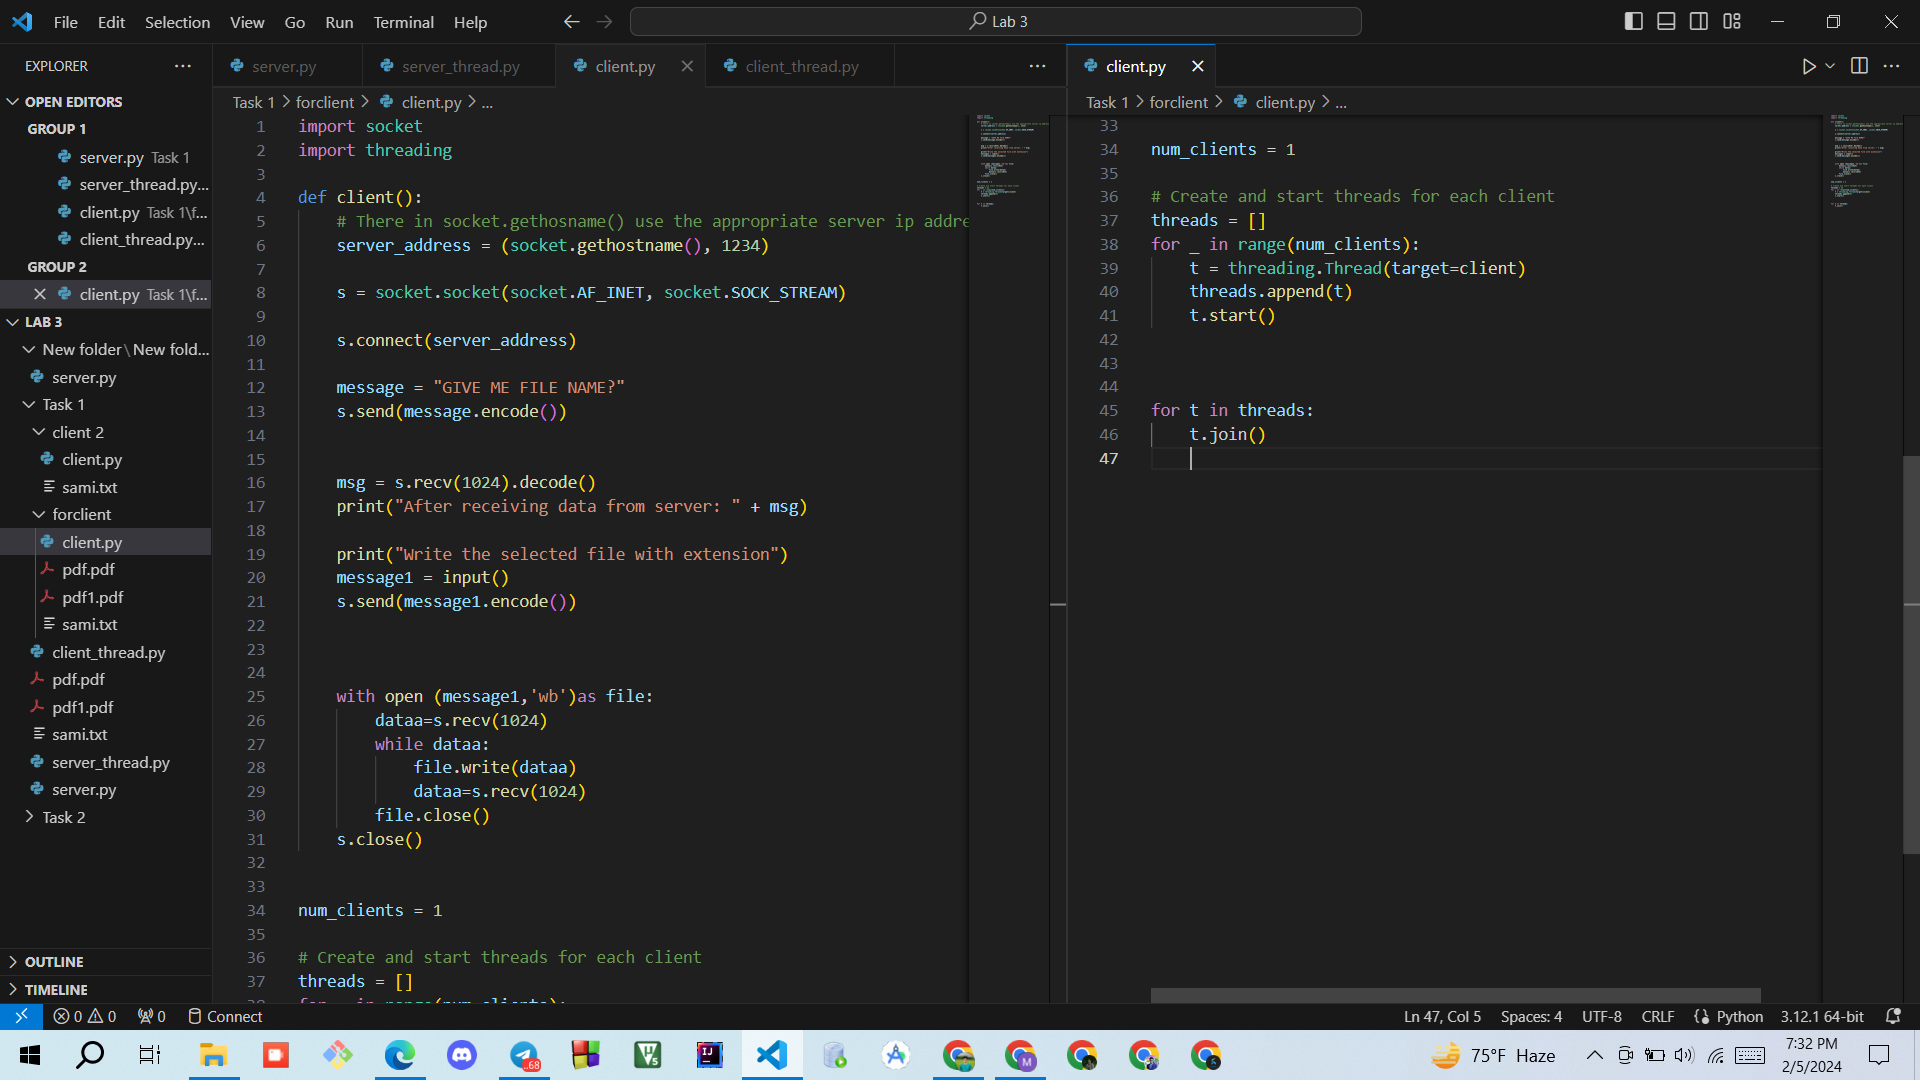
\includegraphics[width=0.8\textwidth]{client.png}
        \caption{Client side code}
        \label{fig:1}
    \end{figure}
    
    \begin{figure}[H]
        \centering
        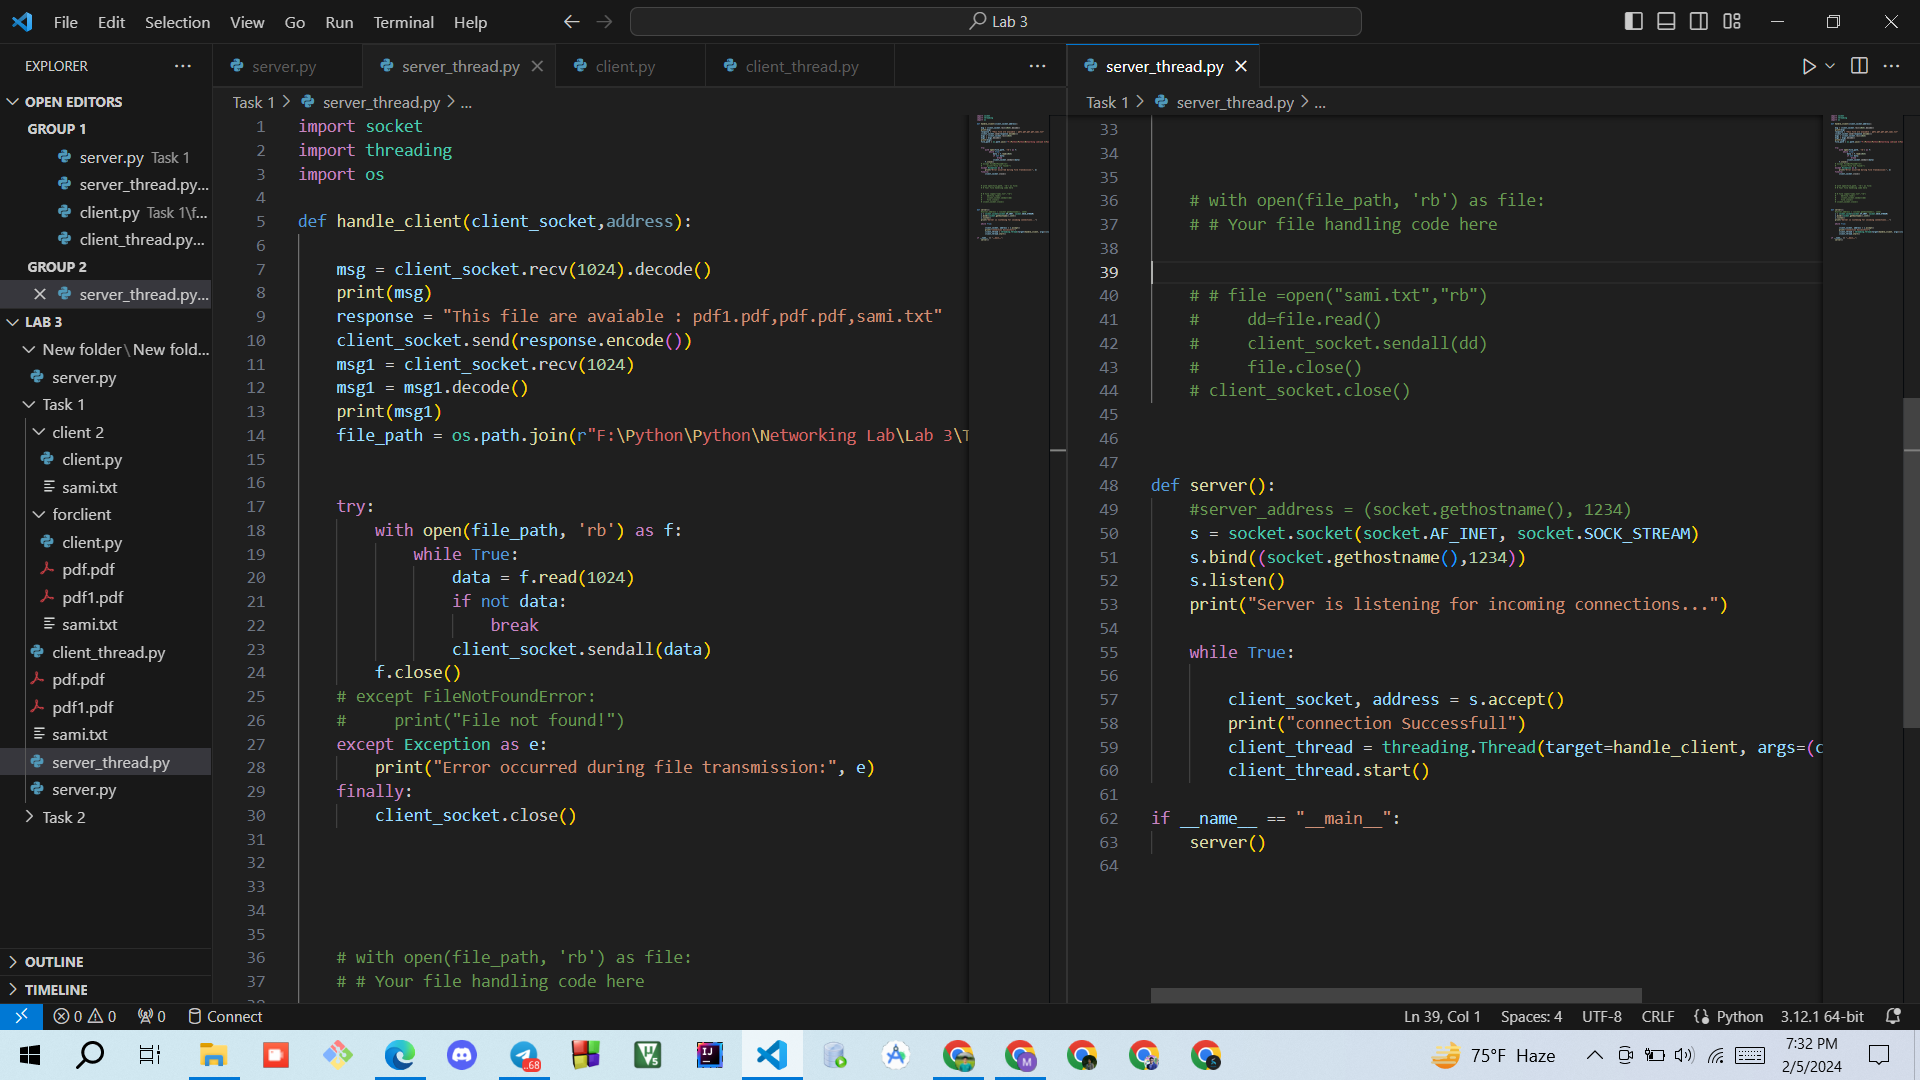
\includegraphics[width=0.8\textwidth]{server.png}
        \caption{Server Side Code}
        \label{fig:2}
    \end{figure}
    
    \begin{figure}[H]
      \centering
      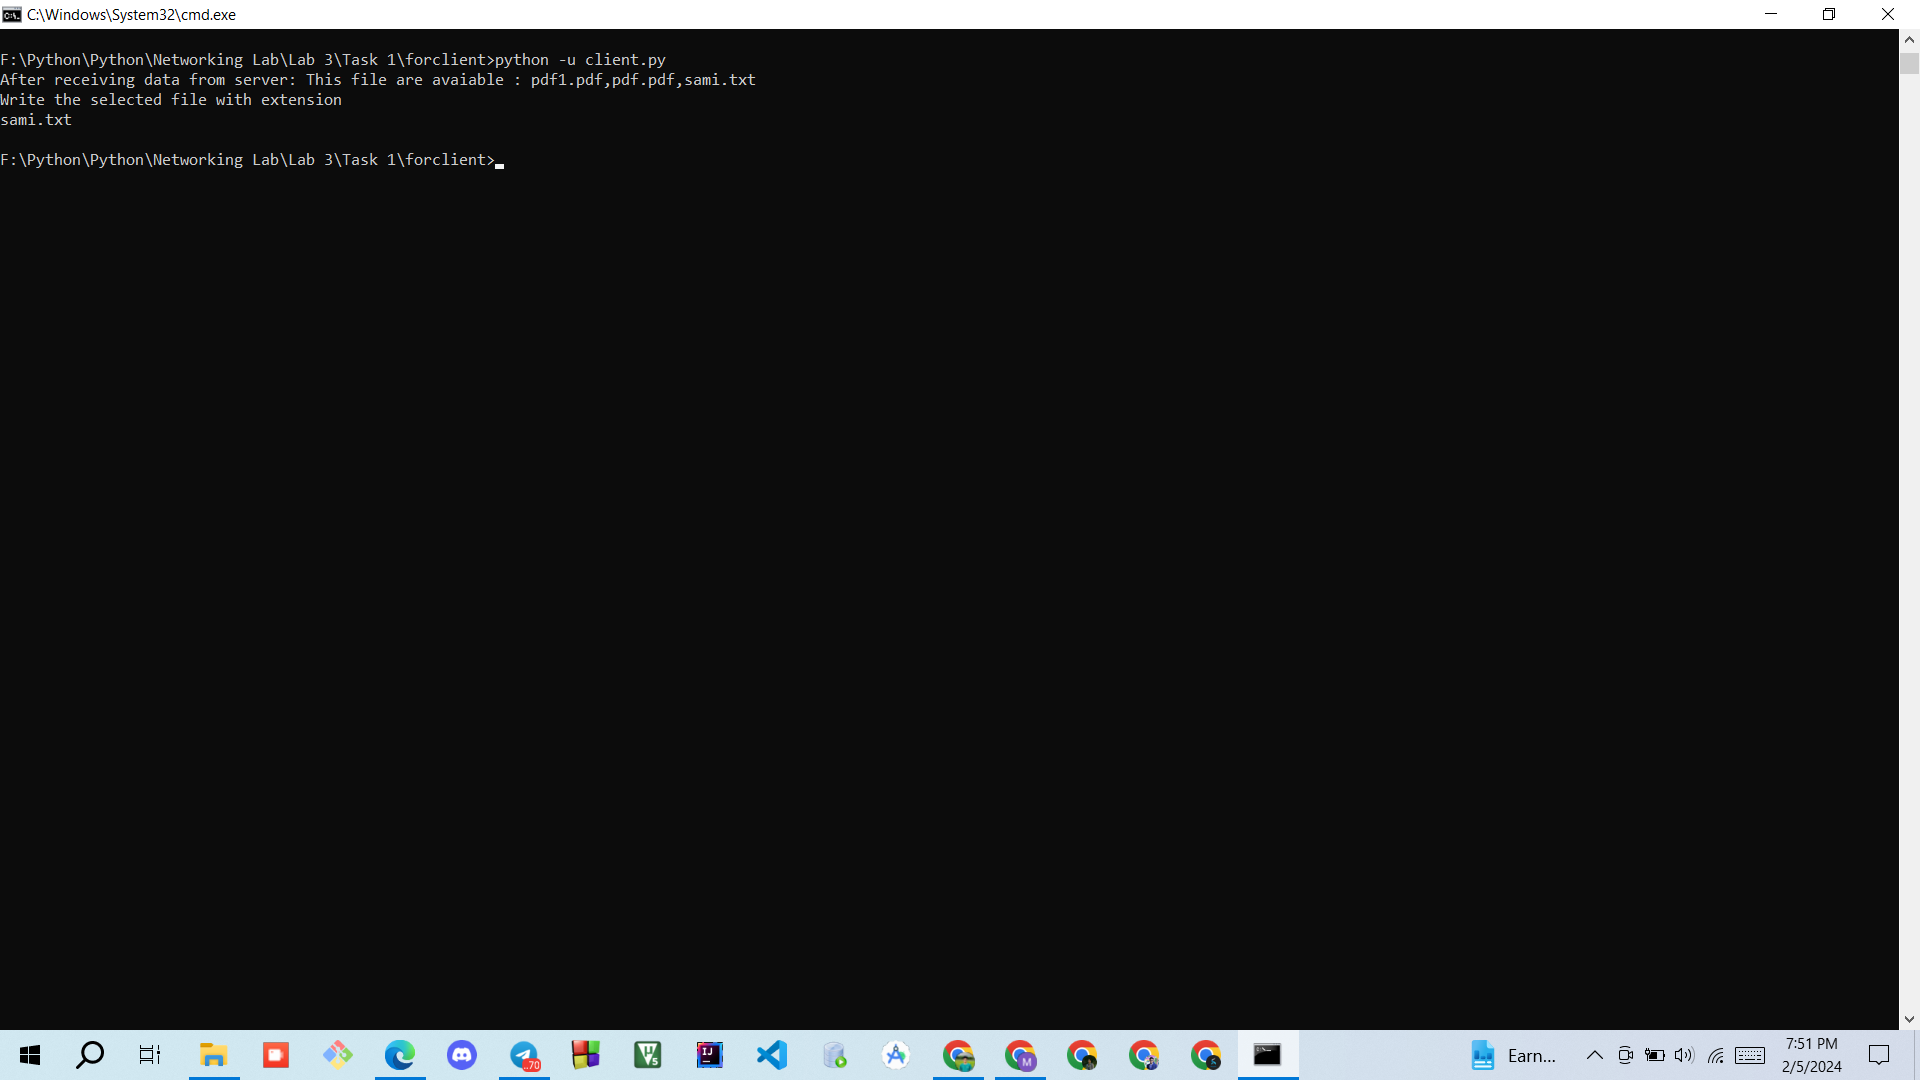
\includegraphics[width=0.8\textwidth]{client_result.png}
      \caption{Client Side result}
      \label{fig:3}
    \end{figure}
    
    \begin{figure}[H]
      \centering
      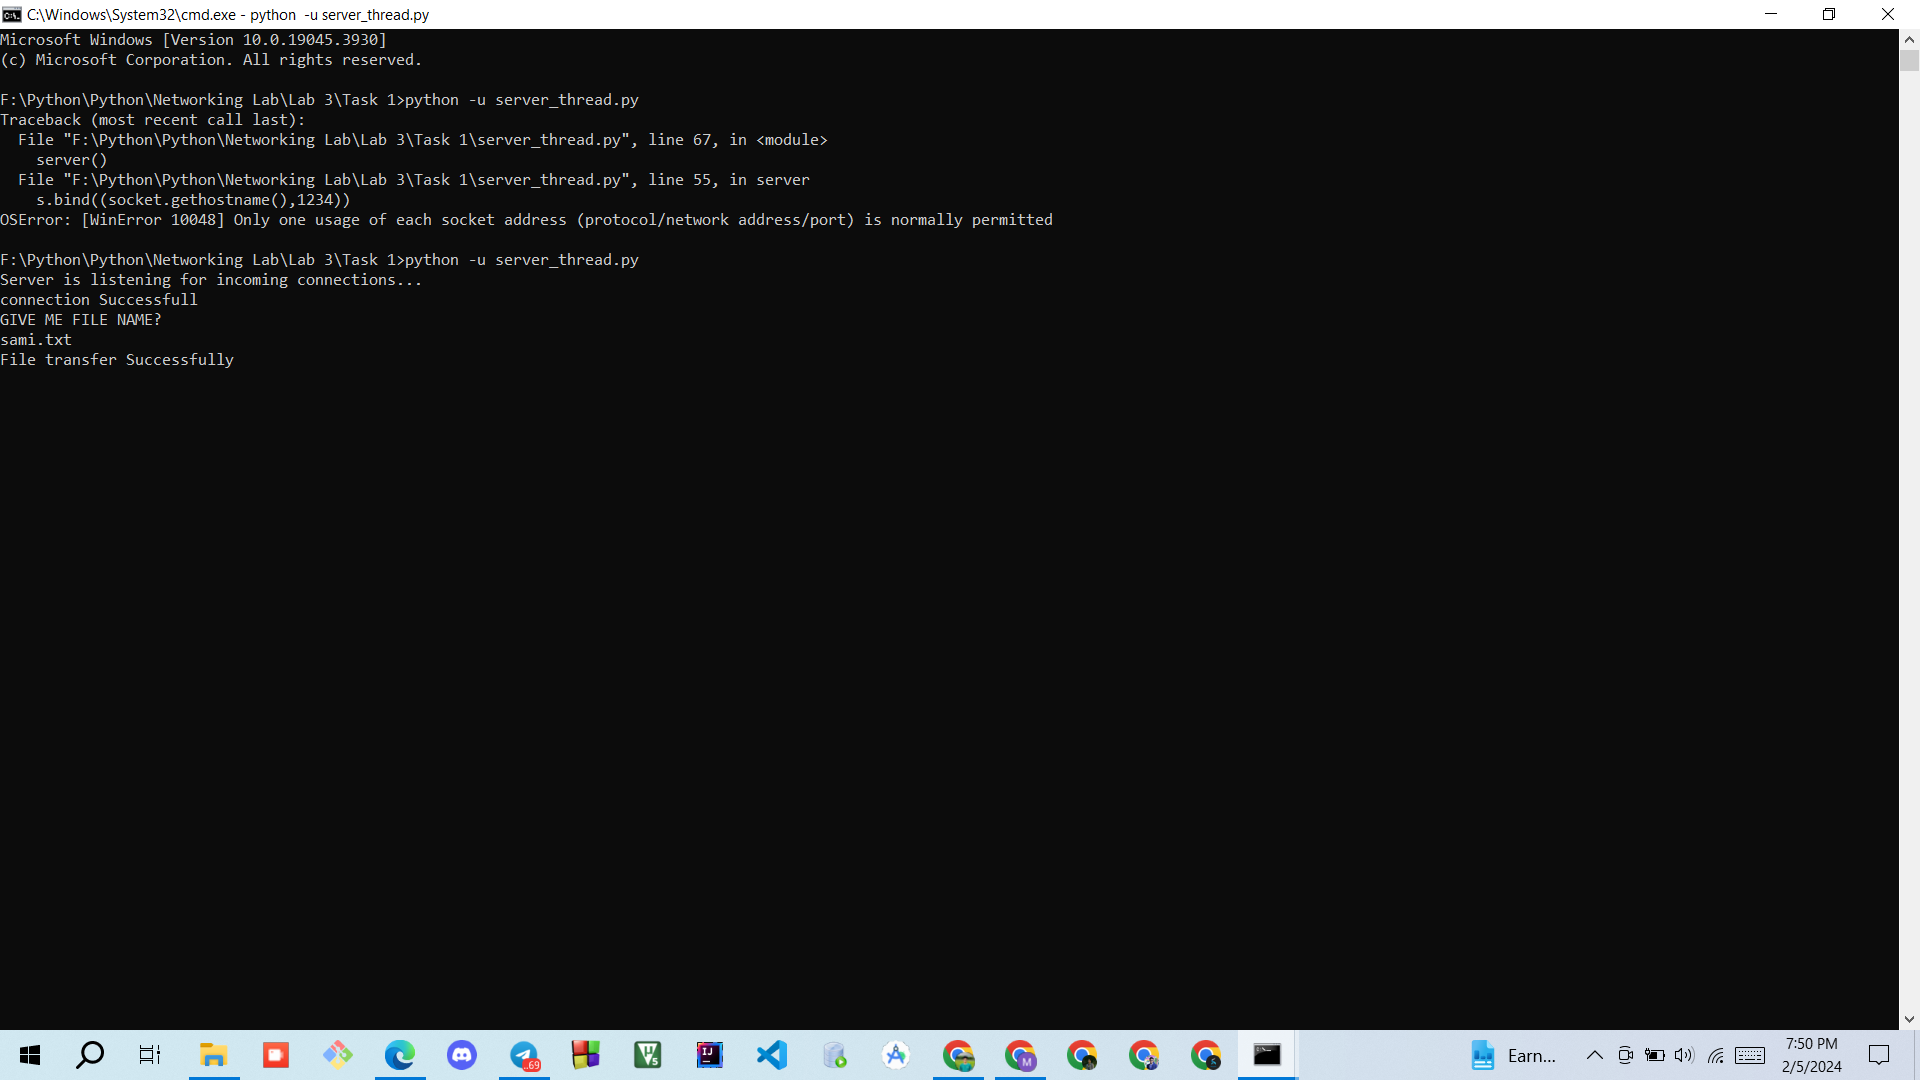
\includegraphics[width=0.8\textwidth]{server_result.png}
      \caption{Server Side result}
      \label{fig:4}
    \end{figure}

\end{itemize}

 
\subsection{Task 2}
\begin{itemize}
\item \textbf{File Transfer via  HTTP handelling multiple clients simultaneously.}
    \begin{minted}[mathescape, linenos]{python}
    SERVER SIDE CODE
    from http.server import BaseHTTPRequestHandler, HTTPServer
import os

class FileServerHandler(BaseHTTPRequestHandler):
    def do_GET(self):
        try:
            
            if self.path == '/':
            
                file_path = 'index.html' 
            else:
                
                file_path = self.path[1:]


            if os.path.exists(file_path) and os.path.isfile(file_path):
                with open(file_path, 'rb') as file:
                    self.send_response(200)
                    self.send_header('Content-type', 'application/octet-stream')
                    self.send_header('Content-Disposition', f'attachment; filename="{os.path.basename(file_path)}"')
                    self.end_headers()
                    self.wfile.write(file.read())
                    print("Client Get Request ")
            
            else:
                self.send_response(404)
                self.end_headers()
                self.wfile.write(b'File not found')

        except Exception as e:
            self.send_response(500)
            self.end_headers()
            self.wfile.write(str(e).encode())

    def do_POST(self):
        try:
            content_length = int(self.headers['Content-Length'])
            file_content = self.rfile.read(content_length)
            
           
            unique_filename = f'received_file_{content_length}.txt'
            
            with open(unique_filename, 'wb') as file:
                file.write(file_content)

            self.send_response(200)
            self.end_headers()
            print("Client Post Request ")
            print("Save it in server disk ")
            self.wfile.write(b'File saved successfully')

        except Exception as e:
            self.send_response(500)
            self.end_headers()
            self.wfile.write(str(e).encode())

def run_server(port=8080):
    try:
        server_address = ('', port)
        httpd = HTTPServer(server_address, FileServerHandler)
        print(f'Starting server on port {port}')
        httpd.serve_forever()

    except KeyboardInterrupt:
        print('Server stopped')

if __name__ == '__main__':
    run_server(port=8080)

   

\end{minted}
    \begin{minted}[mathescape, linenos]{python}
    CLIENT SIDE CODE
   import requests

def download_file(url, save_path):
    response = requests.get(url)
    
    if response.status_code == 200:
        with open(save_path, 'wb') as file:
            file.write(response.content)
        print(f'Downloaded file: {save_path}')
    else:
        print(f'Error downloading file. Status code: {response.status_code}')

def upload_file(url, file_path):
    with open(file_path, 'rb') as file:
        files = {'file': (file_path, file)}
        response = requests.post(url, files=files)

    if response.status_code == 200:
        print(f'File uploaded successfully to {url}')
    else:
        print(f'Failed to upload file. Status code: {response.status_code}')

if __name__ == '__main__':
    server_url = 'http://localhost:8080'

    # Example: Downloading a file
    download_file(f'{server_url}/request_download.txt', 'downloaded_file.txt')

    # Example: Uploading a file
    upload_file(server_url, 'upload_from_client.txt')

\end{minted}

\begin{itemize}
    \item \textbf{}
    
  . 
    \begin{figure}[H]
        \centering
        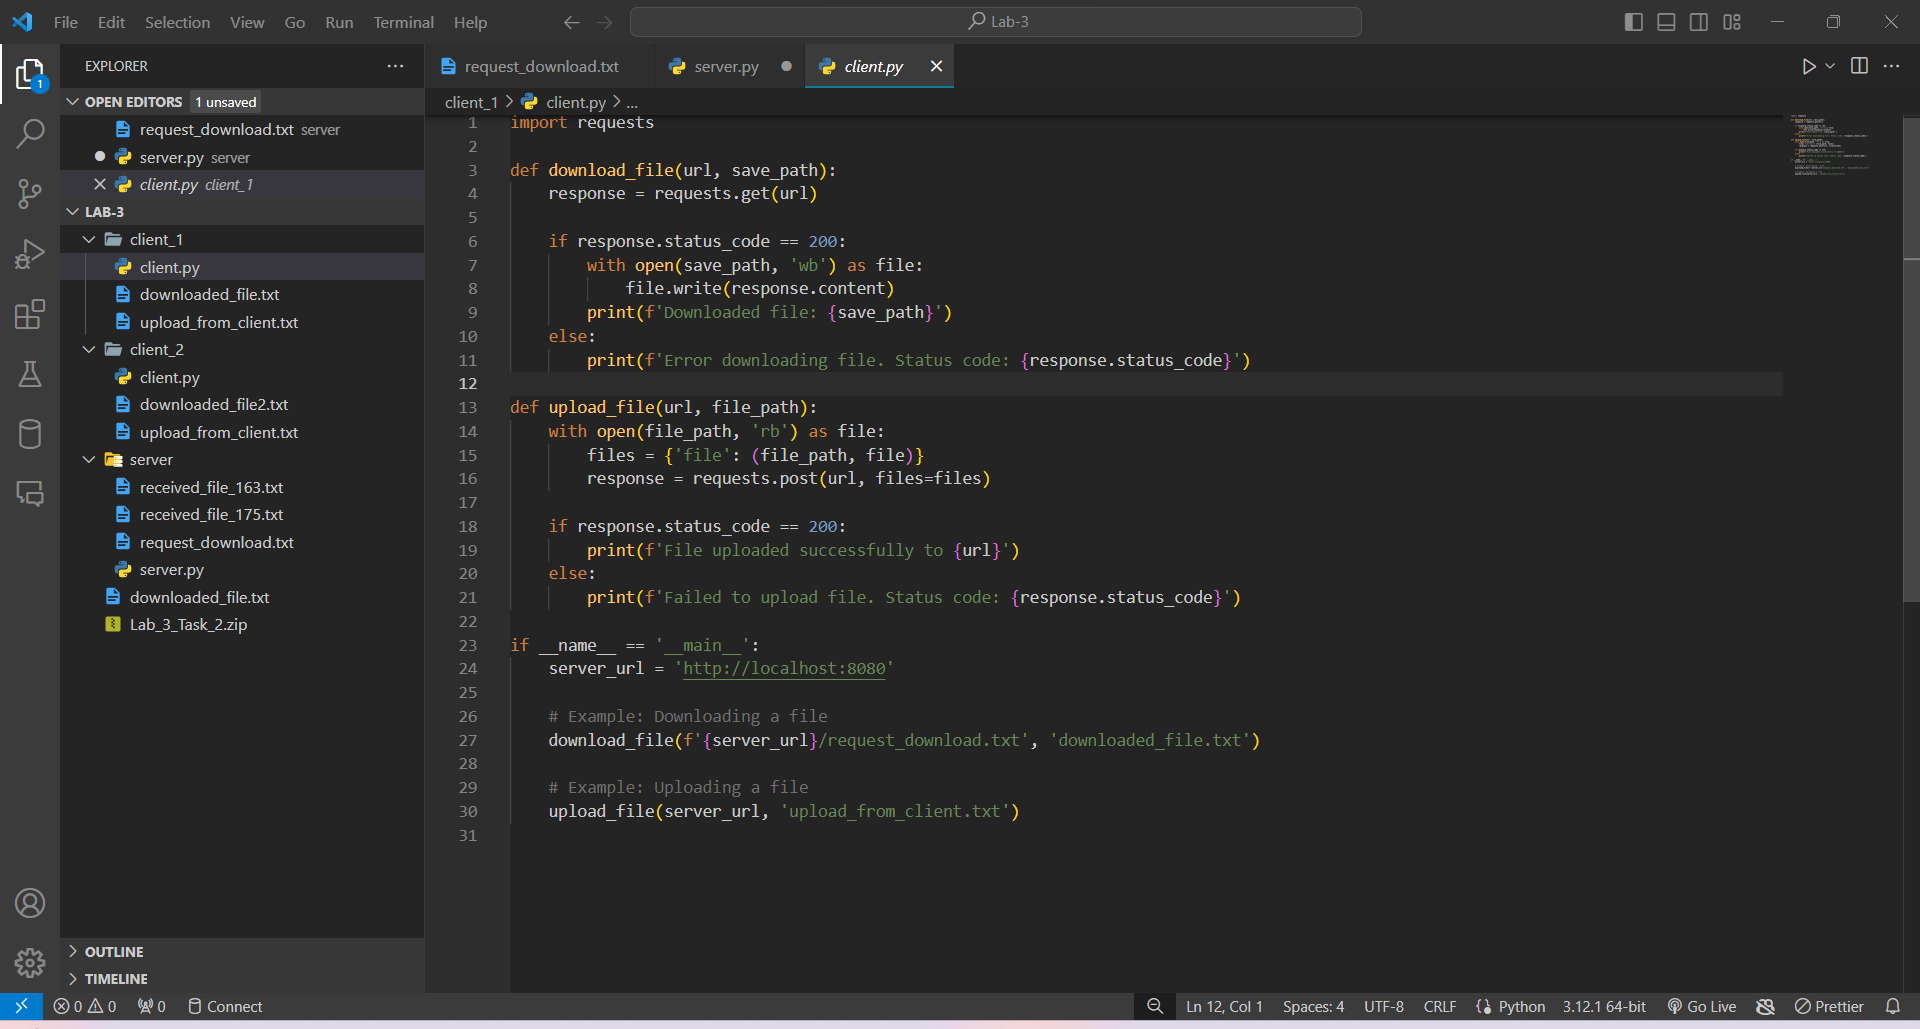
\includegraphics[width=0.8\textwidth]{client2.png}
        \caption{Client side code}
        \label{fig:1}
    \end{figure}
    
    \begin{figure}[H]
        \centering
        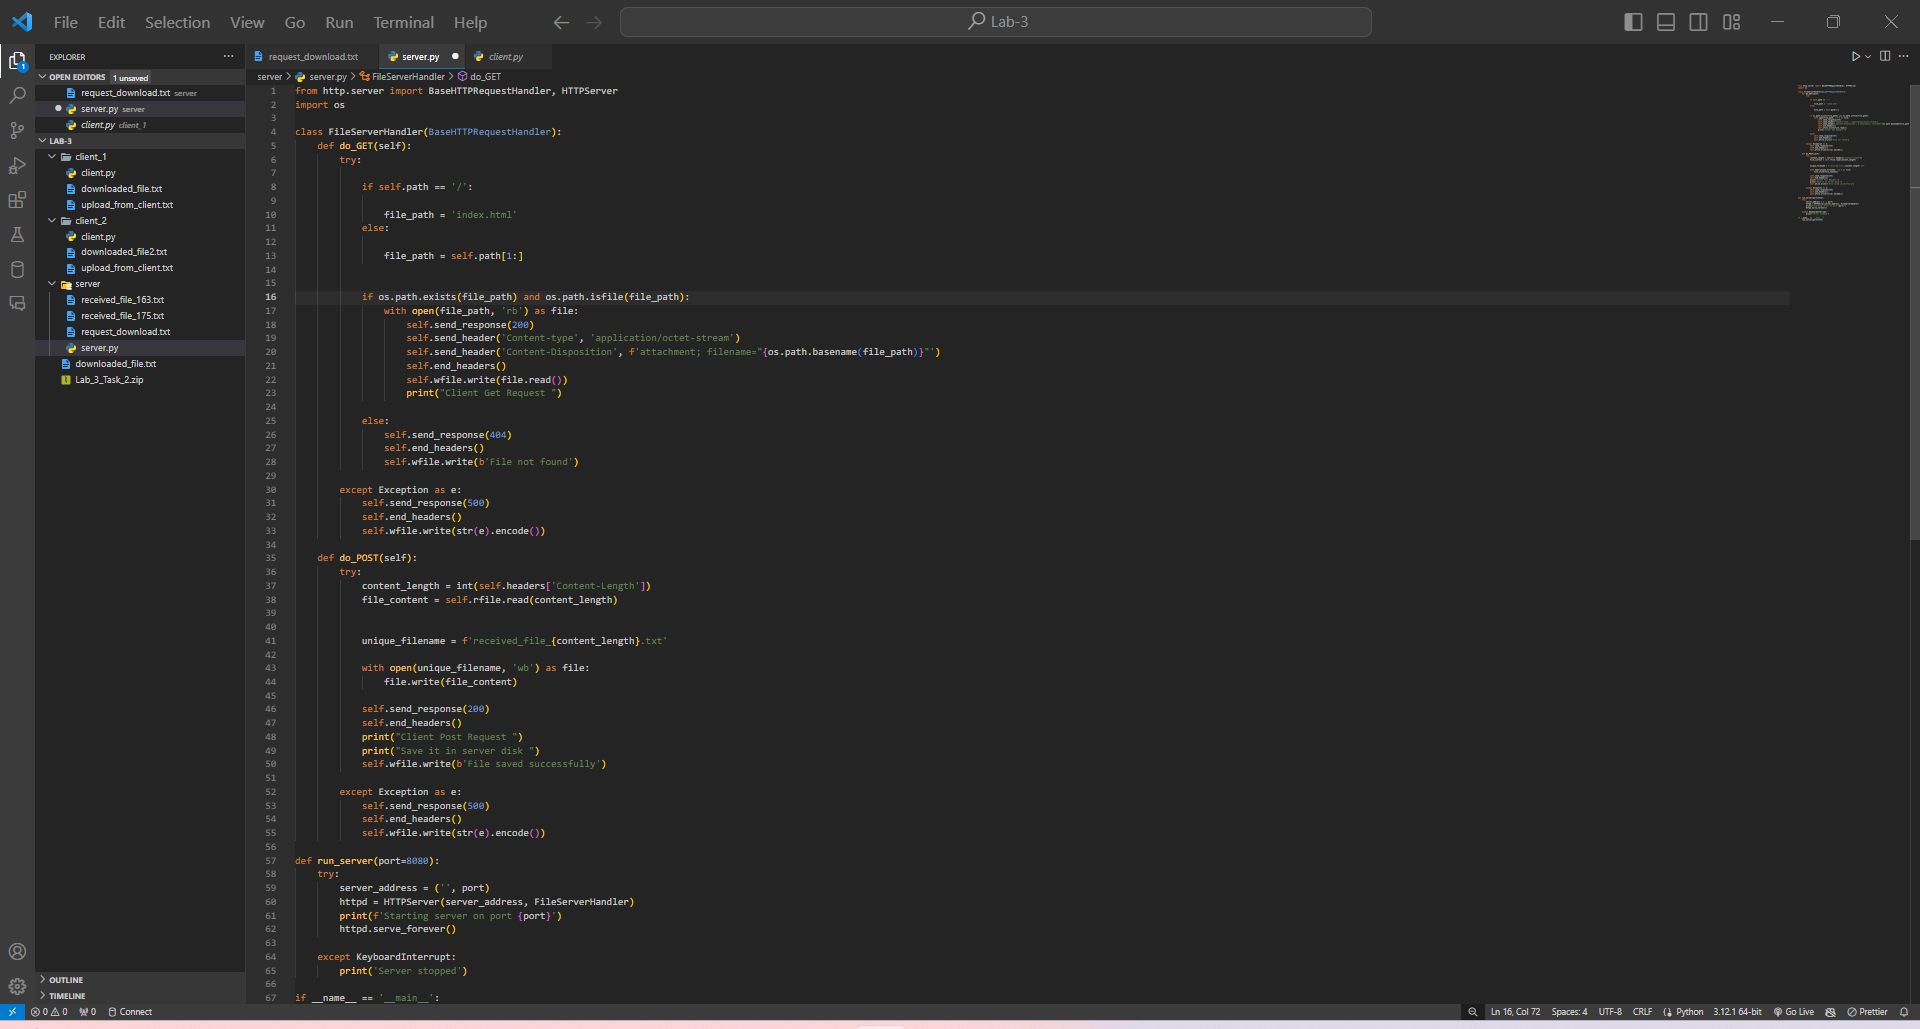
\includegraphics[width=0.8\textwidth]{server2.png}
        \caption{Server Side Code}
        \label{fig:2}
    \end{figure}
    
    \begin{figure}[H]
      \centering
      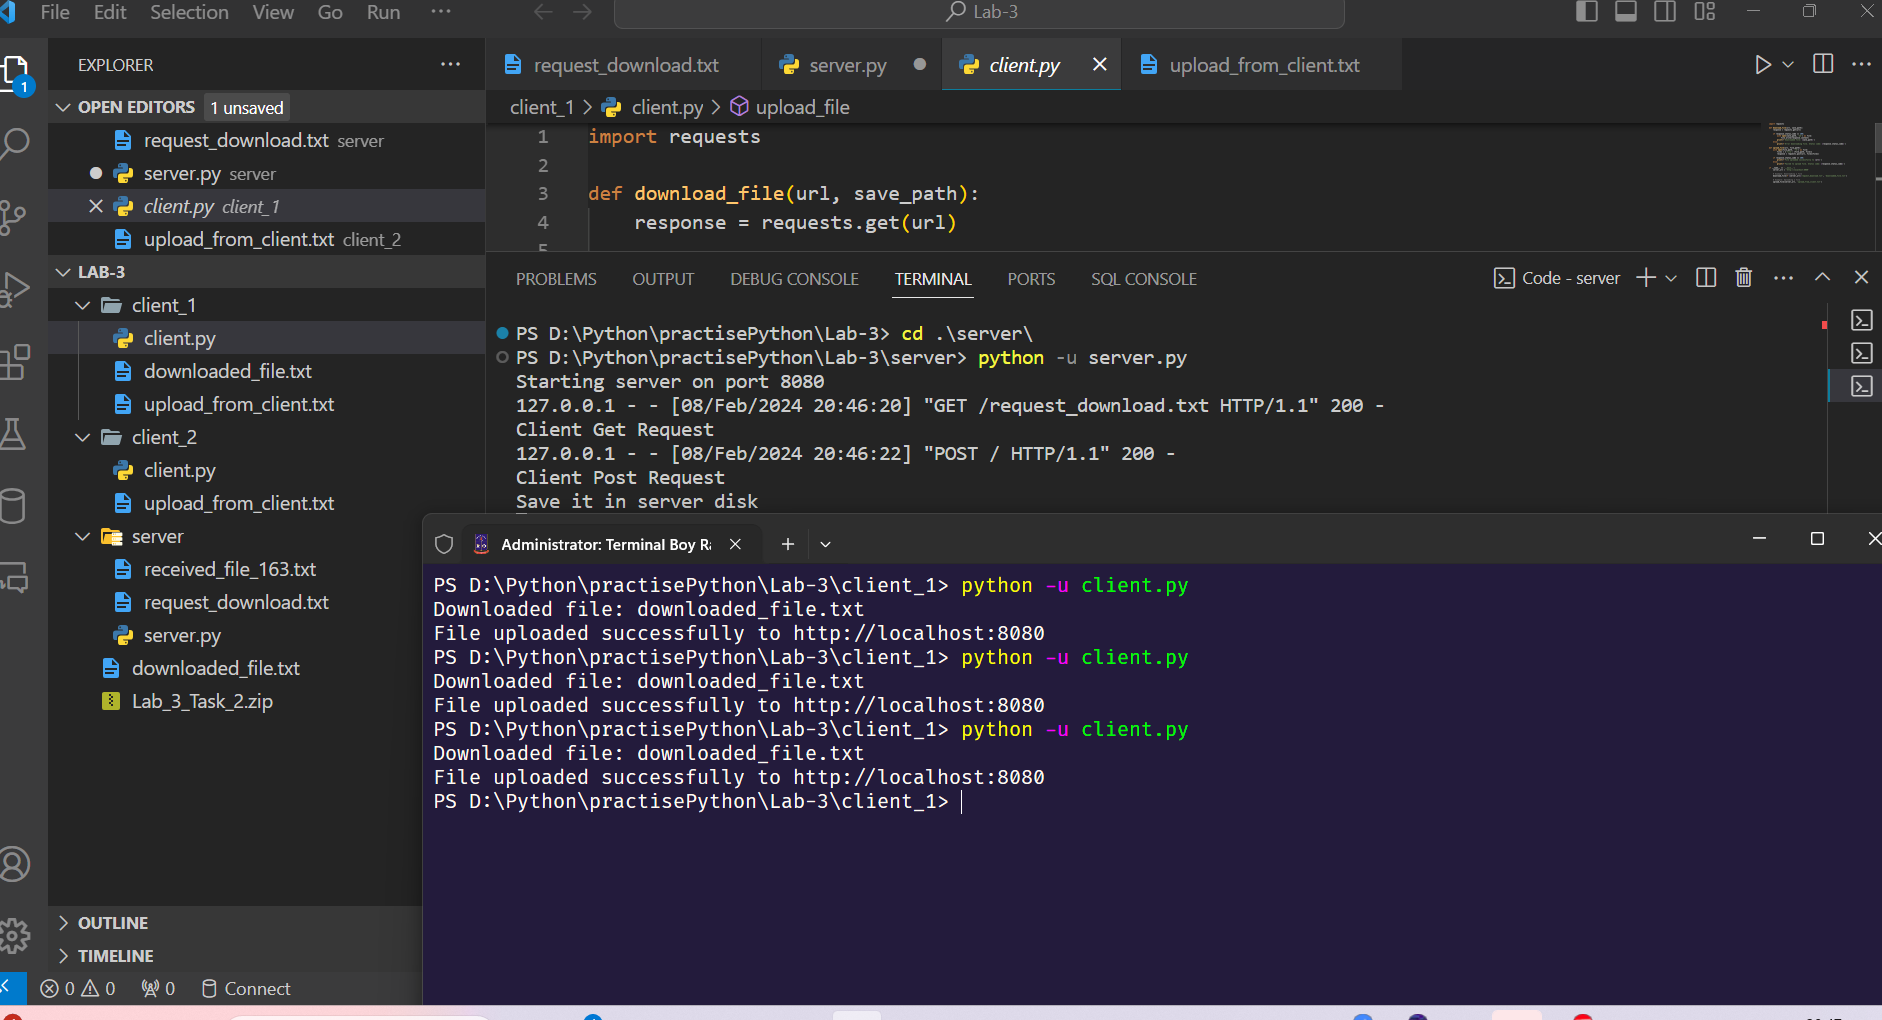
\includegraphics[width=0.8\textwidth]{single_client_result.png}
      \caption{Result for Single client}
      \label{fig:3}
    \end{figure}
    
    \begin{figure}[H]
      \centering
      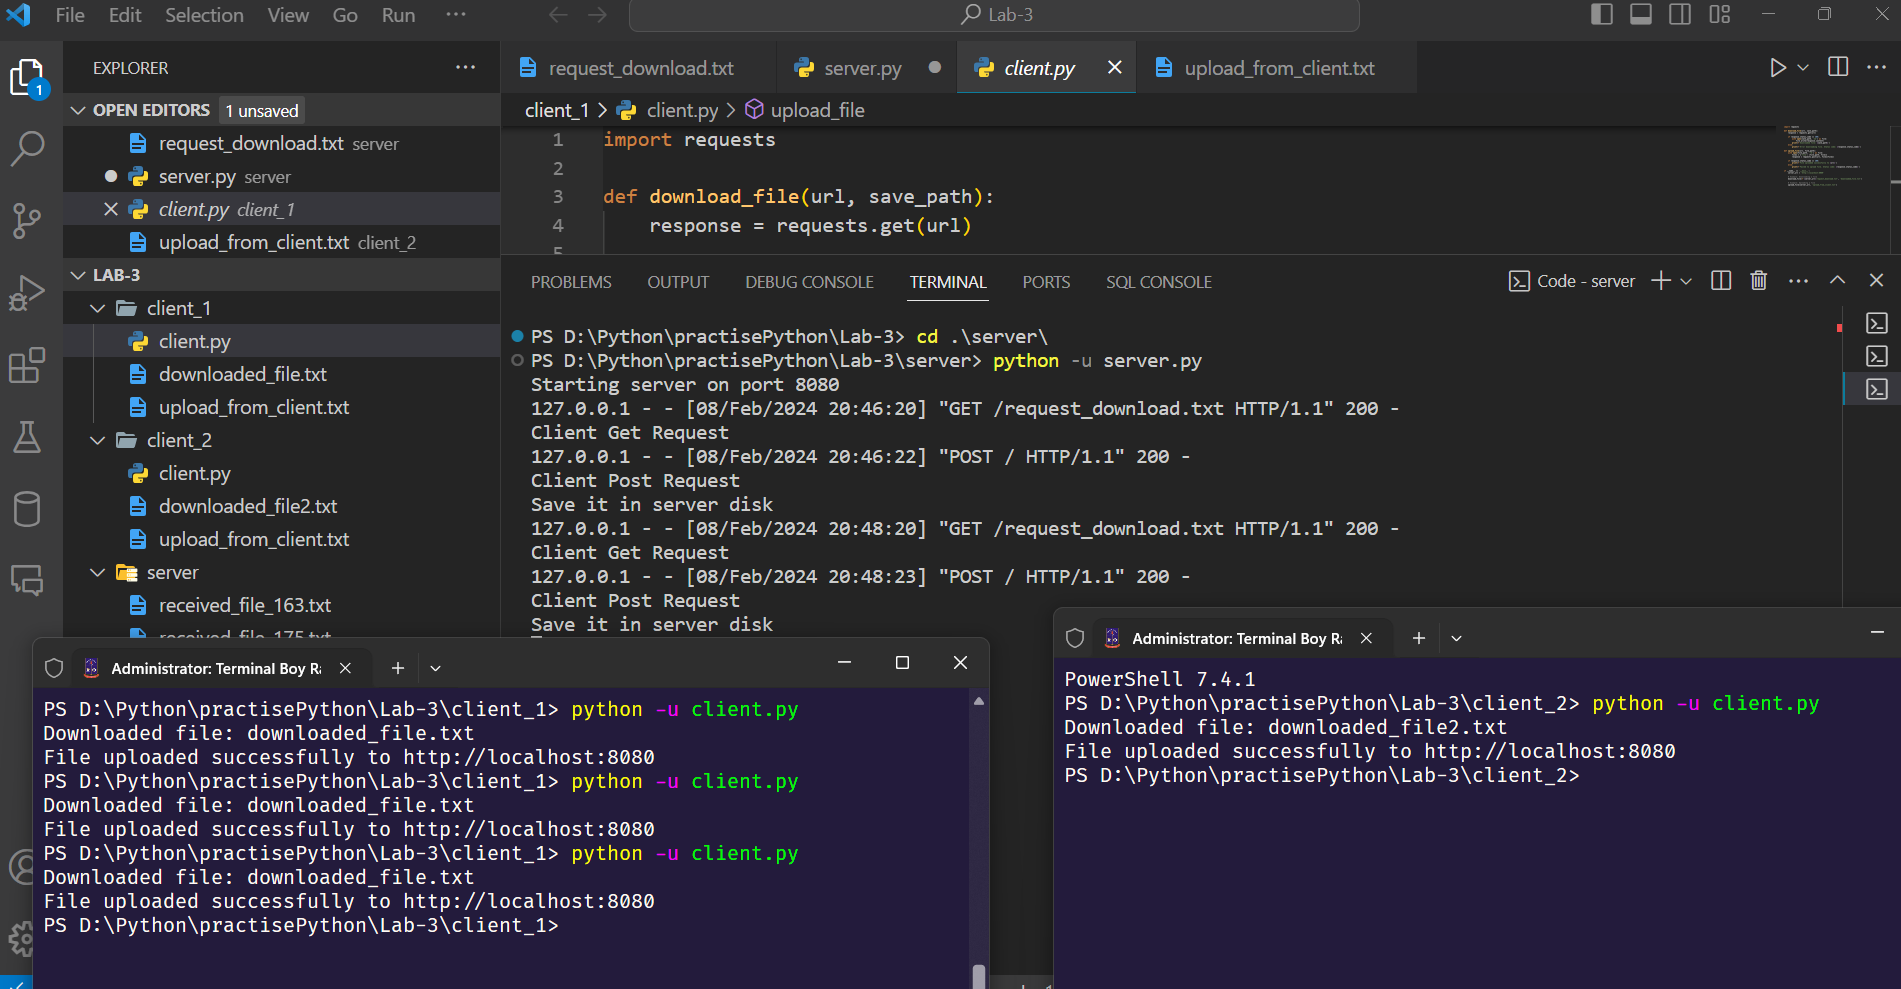
\includegraphics[width=0.8\textwidth]{multiple_client_result.png}
      \caption{Result for multiple client}
      \label{fig:4}
    \end{figure}

\end{itemize}





\newpage
\section{Experience}
\begin{enumerate}
    \item  Ensuring that the server and client handle user inputs safely and validate file paths and names.
    \item We have create multiple clients , thats why we needs more than one terminal 
     for clients side and one for server sides
    \item First we run server side program and then client request server for specific task
    \item Server handle multiple clients  request simultaneously, using treads programming 
    \item Handling different HTTP methods: Supporting both GET and POST methods for file transfer.
    \item Identifying and resolving issues related to socket communication, file handling, or HTTP protocol implementation.
\end{enumerate}





\begin{thebibliography}{1}
  %\bibitem{book} Computer networking: a top-down approach 6th ed.
  \bibitem{geeksforgeeks} Socket Programming in Python: \url{https://www.geeksforgeeks.org/socket-programming-python/}
  \bibitem{realpython} Socket Programming in Python: \url{https://realpython.com/python-sockets/}
  \bibitem{freecodecamp} File Transfer via HTTP: \url{https://www.freecodecamp.org/news/simplehttpserver-explained-how-to-send-files-using-python/#:~:text=Open%20browser%20and%20type%20in,settings%20on%20the%20first%20computer.}
  \bibitem{youtube} File Transfer via HTTP: \url{https://www.youtube.com/watch?v=DeFST8tvtuI&t=630s}
\end{thebibliography}



\end{document}
